\chapter{Analytical modeling}
\thispagestyle{empty}

{\texttt{2018} -- \texttt{2019}}
\bigskip
\smallskip
\label{am}

\section{Introduction}

The main idea is to describe a sound object by analyzing its constituent elements in order to reveal structure characteristics, and use it in terms of composition.
These analysis procedures depend on and are based on the segmentation of the musical object in terms of symbolic elements.

\smallskip

Axiomatic discrimination in terms of irreducible segmentation of an object is an unanswered question in term of the philosophy of science. At least, there is no definitive answer, and we have to deal with the best solution, which remains often unsatisfying, especially when we are talking about human sciences. So, the discrimination is empirical and depends essentially on the analytic and cultural context, and which level of abstraction we are working on \citep{sn}, in other words the axiomatization depends on what one seeks and how one seeks it.

\begin{figure}[!hbt]
	\begin{center}
		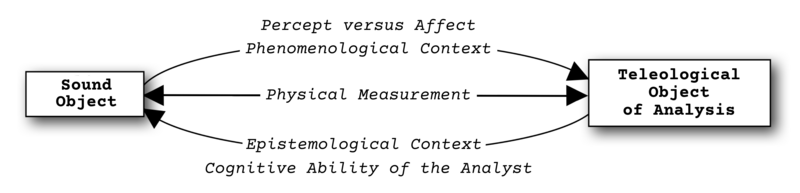
\includegraphics[width=\columnwidth]{img/7583}
		\caption{Synaptic diagram showing relationships of the sound object relative to the analyst.}
		\label{fig:sdqq}
	\end{center}
\end{figure}

Then, Encoding presupposes an interpretation in terms of \textit{percept} -- including \textit{affect} -- of the sound phenomenon considered, such as the teleological object of analysis in the musical context induces a qualitative or a quantitative axiomatization. The second can be derived from the first by empirically associating numerical values with a quality recognized as such, validating the relevance of the observation. The qualitative character depends on the phenomenological context and the cognitive ability of the analyst implying an \textit{in situ} relationship -- even an interaction -- between the sound object and the analytical design of the model (see diagram on figure \ref{fig:sdqq}). Note that the cognitive ability of the analyst fits into the \textit{\'epist\'em\`e} \citep{mflmelc}.
	
The type of encoding is then decisive and depends on the analytic perspective considered.

\bigskip

This is one proposition for automatic analysis as modeling in a musical context and from a sound file in terms of difference and resemblance. Some steps are inevitably empirical, and the modeling is somehow more about optimization of computation as resolutions of combinatorial issues.

This work falls within the margin of the project \textsl{Neuromuse3} and it has been inspired by the research report \textit{Morphologie} \citep{mp}.

\section{Encoding}

The encoding consists to identify useful and isolable component -- with algorithmic or symbolic discriminative processes -- as the axiomatic of the studied system. This is always done in the teleological perspective of analysis and synthesis. 
Note that the musical object represents an abstractive level from the axiom to the whole object as a system.

\begin{figure}[!hbt]
	\begin{center}
		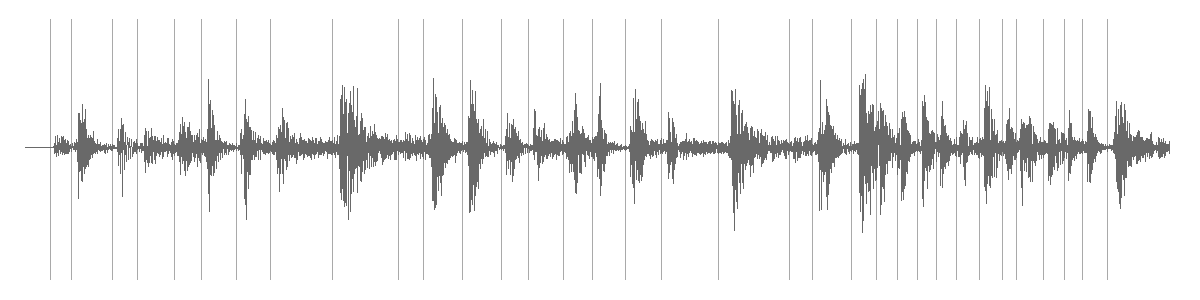
\includegraphics[width=\columnwidth]{img/3790}
		\caption{The waveform of the 5 first seconds of the sample with its associated segmentation according to the TextGrid generated 
		%by the previous command
		with
		 \textsl{enkode}. [ $\rightarrow$ \ref{an:wav} ]}
		\label{fig:wave}
	\end{center}
\end{figure}
	
\textbf{\textsl{enkode} analysis}
\smallskip

The aim of this encoding is to normalize data from a sound file using the analytic tools of the software Praat managed by the command line \textsl{enkode}, defined as a multidimensional array of 5 dimensions. This array contents the duration, $f0$, centroid, loudness and `loudbass'.

\smallskip

\begin{lstlisting}[language=bash]
$ enkode --as-int=3 test.mp3 > test.dat
\end{lstlisting}

\section{Symbolisation}
\label{sym}

\textbf{Hierarchical clustering}
\smallskip

The hierarchical clustering of the previous multidimensional data is built inside the artificial neural network \textsl{Neuromuse3} context -- called CAH -- according to the output of the neurons as events. The agglomerative process use the Euclidean distance.

\smallskip

\begin{lstlisting}[language=Lisp]
CL-USER> (require 'N3)
CL-USER> (in-package :N3)
N3> (defvar *DATA* (remove-duplicates (read-file "test.dat") 
     :test #'equalp))
N3> (create-mlt 'test (length (car *DATA*)) (length *DATA*) 
     :carte #'rnd-map)
N3> (loop for neuron in (neurons-list test) 
     for dat in *DATA* do (setf (output neuron) dat))
N3> (dendrogram test 3 :and-data t)
;; The second argument is the aggregation type :
;; Ward's method in this case
-934.9051+
\end{lstlisting}

\smallskip

The function \texttt{dendrogram} generates a data file with the number of nodes according to the trimming distance associated with the minimum distance of the parent node and the sum of the intra-class inertia of the children nodes of the parent node.

Now, the idea is to get the optimum number of classes according to the distance from the parent node and the intra-class inertia. There are no rules, therefore the choice is empirical and estimated with the degree of accuracy analysis required. All it needs to be know is that the distance has to be maximum and the inertia minimum.

However, in \textsl{Neuromuse3} context, the optimization can be done according to the number of the current \textit{`fanaux'} in order to be more accurate by increasing their number.

\begin{figure}[!hbt]
	\begin{center}
		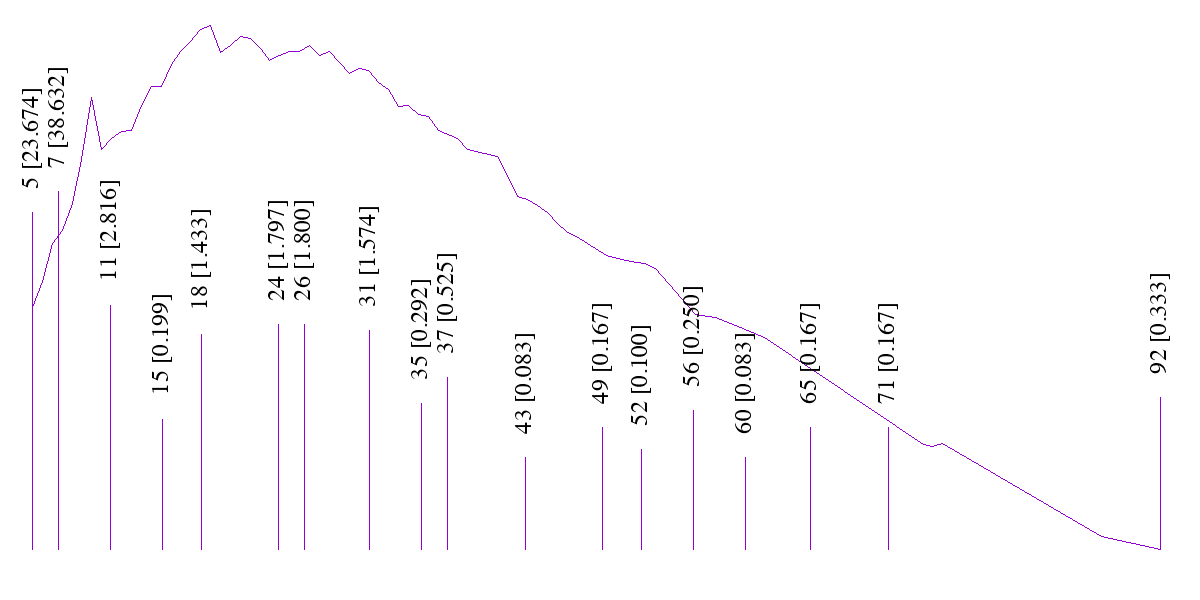
\includegraphics[scale=0.35]{img/4412}
		\caption{The curve is the sum of the intra-class inertia by trimming. The lines are the peaks of the curve of minimum distance from the parent node (as the second number in the square bracket, the first number is the number of classes at this point). 
		%Note that in this graph, the inertia curve is scaled on the y-axis with the impulse segments in order to fit on the same diagram.
		Note that in this graph, the impulse segments are displayed in a logarithmic scale for better readability.}
		\label{fig:seg}
	\end{center}
\end{figure}
	
In this case, this is a segmentation of 5 classes -- referred to as A, B, C, D, and E -- which is retained as result.

\smallskip

\begin{lstlisting}[language=Lisp]
N3> (alpha-seq test -934.9051+ 5 (read-file "test.dat"))
(C C C A A C C D D A C B C A A E C D D A C A A B B B B B B E 
 B B B D A C A A E B B B B B E E B B B B A C D E A A E A A C
 B B B B E A A A A B B A D A B C C A C E C D D A C D B A E C
 D A A A B B E A A E B A D A E D E A A E A D D C C B E A B B
 C E B D A B D A A E B A A A B B E A A B C D B B)
\end{lstlisting}

\section{Contrastive analysis}

\textbf{Segmentation by marker}
\smallskip

The contrastive analysis consists to segment an array of symbol according to a marker defined by the number of occurrences of this marker as a smallest sub-structure, or in other words according to the number of repetitions and for a short sequence which is more focused by the brain as a relevant marker to memorize. This is done recursively until all symbols are different. The side effect of this algorithm is, in the case of strict equality between different occurrences of sequences, the choice is done according to the sorting algorithm of the lisp implementation, which we retain the first item. The function \texttt{structure-s} takes as argument the symbolic sequence previously computed.

The two last merging affect sequentially -- that is to say on the whole sequence -- two adjacent items respectively if the first is equal to the head of the second (for instance the sequence \texttt{AB ABC} becomes \texttt{ABABC}), and if the second is equal to the tail of the first (for instance the sequence \texttt{ABC BC} becomes \texttt{ABCBC}).

\begin{lstlisting}[language=Lisp]
N3> (structure-s (alpha-seq test -934.9051+ 5  
     (read-file "test.dat"))) 
(CCC AACC DDACBC AAEC DDACAA BBBBBB EBB BDAC AAEBB BBB EE
 BBBBACDEAAEAA CBB BBEAA AABBAD ABCC ACEC DDACDBAE CDAA
 ABBEAAEBAD AE DEAA EAD DC CBE ABBC EBD ABDAA EBAA ABBEAABC 
 DBB)
\end{lstlisting}

\section{Paradigmatic analysis}
\label{paradigm}

\textbf{Unrooted tree}
\smallskip

The paradigmatic analysis allows to observe typological variations within an object or a corpus.

There are no rules either for the paradigmatic discrimination, but an analysis by hierarchical clustering with the single linkage or the complete linkage as aggregation can offer some guidelines.

With this approach, we can accurate the proximity between 'sub-structures' according to the current musical context. The main idea is to use the Levenshtein distance with some preliminary algorithms which are respectively defined by the distance according to the local repetition, and the distance between two bijective sequences as patterns $a$ and $b$ according to the decomposition into permutation cycle \citep{pc} -- called $\sigma$ -- defined by $c = | O\sigma(x) |$, such as $\delta(a,b) = | lcm(c_a) - lcm(c_b) |$.

\smallskip

Let $A$ and $B$ be sub-sequences, the distance between $A$ and $B$ is computed as follow :
\begin{enumerate}
  \item Remove common local duplicate(s) such as $A \rightarrow A'$ and $B \rightarrow B'$\\ Then the `repetition distance' is $d_1 = | A \setminus A' | + | B \setminus B' |$
  \item Remove pattern such as $A'' = A' \setminus C$ and $B'' = B' \setminus C$ with $C = A' \cap B'$\\ Then the `transposition distance' is applied to the pattern $C$ as $d_2$
  \item Apply Levenshtein distance between $A''$ and $B''$ as $d_3$
\end{enumerate}

Then the total distance is $d_1 \times w_1 + d_2 \times w_2 + d_3 \times w_3$ with $w_i$ as weight respectively $1/2$, $1/2$ and $1$ by default.

\smallskip

The setting -- that is to say the aggregation type (single or complete linkage) and the weight of each algorithm applied to estimate proximity -- remains empirical but the investigation field is significantly reduced and rather intuitive to integrate this modeling into an automatic process.

\smallskip

\begin{figure}[!hbt]
	\begin{center}
		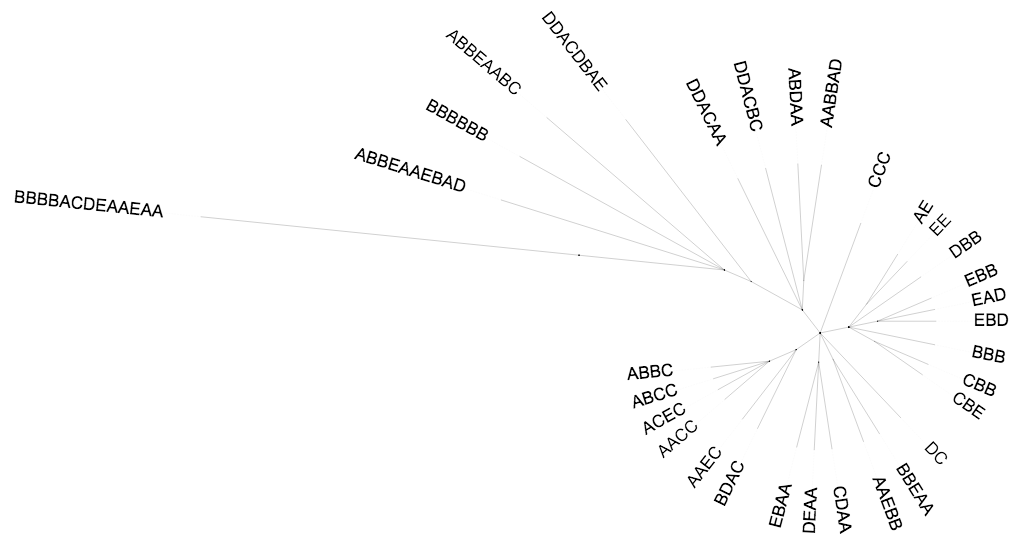
\includegraphics[scale=0.47]{img/5521}
		\caption{Single-linkage clustering.}
		\label{fig:hc1}
	\end{center}
\end{figure}
	
\begin{figure}[!hbt]
	\begin{center}
		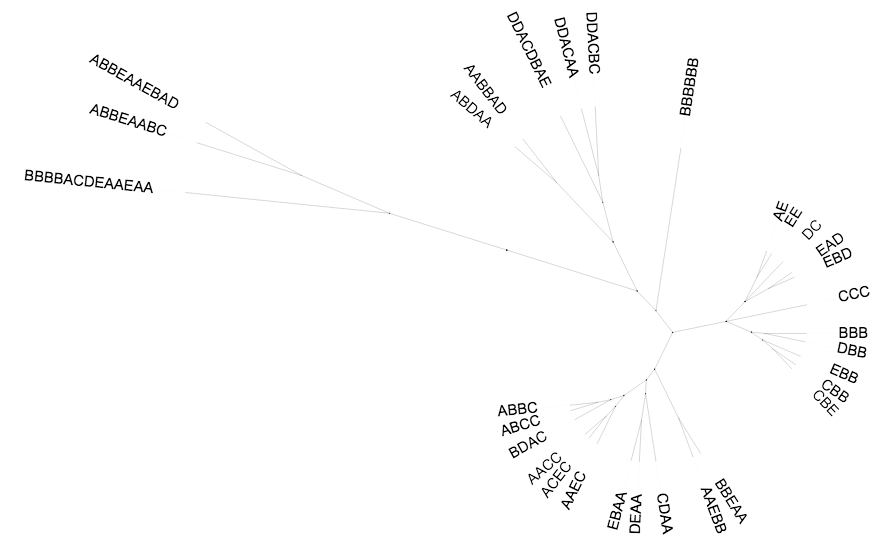
\includegraphics[scale=0.48]{img/5522}
		\caption{Complete-linkage clustering.}
		\label{fig:hc2}
	\end{center}
\end{figure}
	
The figures \ref{fig:hc1} and \ref{fig:hc2} point out the possible groupings with the single and the complete linkage methods. These figures were generated with the online application iTOL\footnote{iTOL allows to display online phylogenetic trees from datasets:\\ \indent \href{https://itol.embl.de/}{\scriptsize{\texttt{https://itol.embl.de/}}}} -- with the display mode set to the unrooted tree --,
from their respective Newick files built from the contrastive analysis as a dendrogram. See appendice \fullref{nwck} for an alternative representation and appendice \fullref{nwdoc} for a description of the standard Newick tree format.

\smallskip
 
\begin{lstlisting}[language=Lisp]
N3> (dendrogram '(CCC AACC DDACBC AAEC DDACAA BBBBBB EBB BDAC AAEBB BBB EE BBBBACDEAAEAA CBB BBEAA AABBAD ABCC ACEC DDACDBAE CDAA ABBEAAEBAD AE DEAA EAD DC CBE ABBC EBD ABDAA EBAA ABBEAABC DBB) 1|2)     
\end{lstlisting}

The single linkage tree can be divided into five paradigmatic fields, while the complete linkage tree offer the possibility to define more obviously four paradigmatic fields. 

In any case, this is the teleologic object which determines the setting, both for the number of discrimination and the way the discrimination is done in terms of distance.

\section{Systemic analysis}

\textbf{Clustering proximity}
\smallskip

Defined as a set of relations that maintain elements between them allowing the constitution of a coherent system. Thus, form and structure are two interrelated notions that determine the immanent or transcendent view of the system.

\smallskip

The form can be expressed in terms of fractality from the micro-form to the macro-form, articulated according to structural modalities, or in terms of recurrence and repetition/variation  \citep{afum}.

In some musical performances, some characteristics involve for a morphogenesis point of view as a dynamic system. Morphogenesis is an `in time' analytic system for observing formal variations according to identified structural processes. Indeed, some traditional musical events for instance are not a piece of music with a determined form, but rather a piece of music that evolves `in time' according to the feelings and some codification in term of proclivity involving each participant.

\smallskip

So, the systemic analysis will focus on the relationship between adjacent sub-structure defined by the contrastive analysis as derivative according to the distance defined for the paradigmatic analysis, and the process of successivity in terms of probability of the elements constituting the sub-structures.

\subsection{Derivative clustering}

\begin{figure}[!hbt]
	\begin{center}
		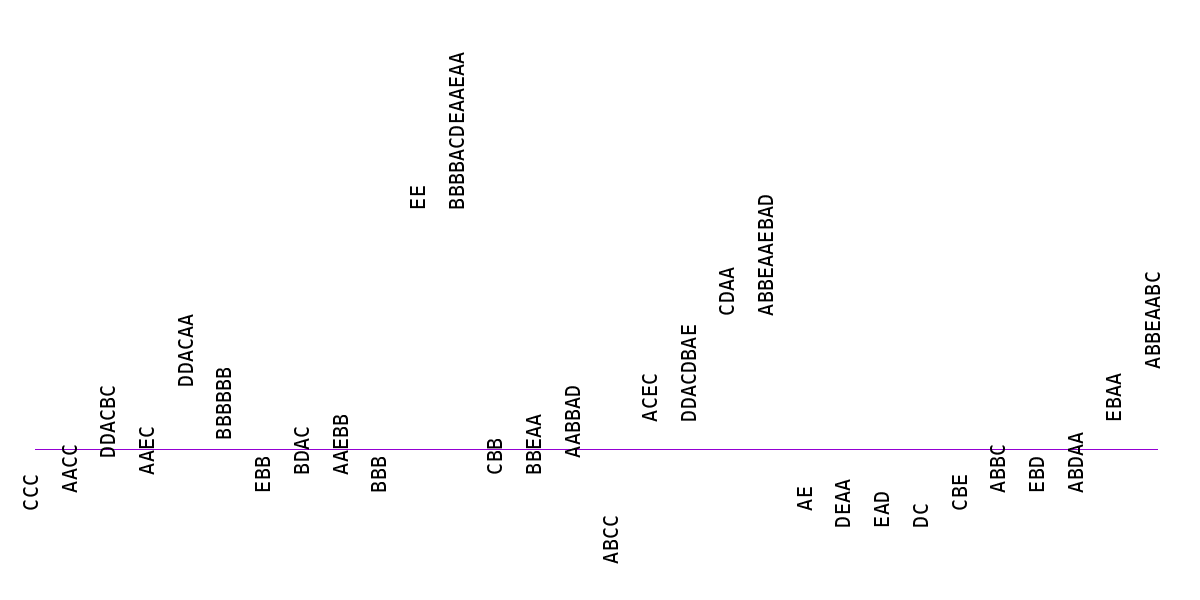
\includegraphics[scale=0.38]{img/8701}
		\caption{The first letter of each sequence marks the distance level -- on the y axis -- to the next sequence. The horizontal line is the mean distance involved all combination of two different sequences.}
		\label{fig:der}
	\end{center}
\end{figure}	

According to the distance between two adjacent sequences, the derivative clustering (see figure \ref{fig:der}) consists to segment the whole sequence into parts `in time' delimited by the mean distance.
	
	\smallskip
		
\begin{lstlisting}[language=Lisp]
;; Thus, the initial sequence is segmented as follow :
N3> (part-s '(CCC AACC DDACBC AAEC DDACAA BBBBBB EBB BDAC AAEBB BBB EE BBBBACDEAAEAA CBB BBEAA AABBAD ABCC ACEC DDACDBAE CDAA ABBEAAEBAD AE DEAA EAD DC CBE ABBC EBD ABDAA EBAA ABBEAABC DBB))
((CCC AACC DDACBC AAEC) (DDACAA BBBBBB) (EBB BDAC AAEBB BBB) 
 (EE BBBBACDEAAEAA) (CBB BBEAA AABBAD ABCC) (ACEC DDACDBAE 
  CDAA ABBEAAEBAD) (AE DEAA EAD DC CBE ABBC EBD ABDAA) (EBAA 
  ABBEAABC))
\end{lstlisting}

\smallskip

Note that the last sub-sequence \texttt{DBB} is omitted because there is no distance defined from this sequence, but this sequence is of course implicitly associated with the last sequence \texttt{ABBEAABC} as distance.

\subsection{Developmental process}

In this analysis, the approach consists to evaluate the probability of an event occurs according to $n$ previous events.
For instance, the probability of events succeeding the sub-sequence \texttt{CD} is :

\smallskip

\begin{lstlisting}[language=Lisp]
N3> (next-event-probability '(C D) (alpha-seq test -934.9051+ 5) :result :verbose)
B => 28.571 %
A => 14.286 %
D => 42.857 %
E => 14.286 %
\end{lstlisting}

\smallskip

Mind that the sum of the probabilities is equal to 100 \%,  or very close according to some rounding error that might be caused by computer systems \citep{re}.

\section{Resolution}
\label{mcres}

During this article, we proceeded to a `deconstruction' of a sample as a sound file -- according to the discriminative analysis of \textit{\textsl{enkode}} as events, and more over as symbols and as sub-structures and their relationship -- with a view to or in the perspective of a `reconstruction' according to for instance a formal grammar defined as a musical L-system \citep{ml}, or a Markov chain, which could be weighted as a developmental process.

\noindent
\begin{info}
\begin{minipage}{0.95\textwidth}
\vspace{0.25cm}
According to the transition probability matrix defined by the function \texttt{next-event-probability}, it is possible to experiment with a Markov chain as follow:
\begin{itemize}[leftmargin=0.45cm]
  \item let $S$ be the initial sequence according to the alphabet $e=\{a,b,c,...\}$ such as $e \subset S$
  \item let $P(e)$ be the probability of an occurrence $e_n$ in $S$
  \item let $w$ be the sub-sequence as the previous state and set with an initial element such as $w=P(e)$ or $w=e_n$ then the next event is $P(e|w)$
  \item if $P(e|w)$ does not exist or if $P(e_n|w)=1^*$ with $|w|>1$ then minimize $i \in ]0, |w[i]|=1]$ such as $\exists i \in \mathbb{N}:P(e|w[i]) \in e$ knowing that $w[i]$ is the position of and from the beginning of the reduced $w$ as a tail sub-sequence, or in other words as a suffix.
  \item if $P(e|w)=1$ with $|w|=1$ then the next event is $P(e)$ in order to avoid an endless loop on a sub-sequence. 
    \vspace{0.2cm}
\begin{spacing}{1.0}
\footnotesize $^*$ In this case and from this event, we have to solve the \textit{max order problem} \citep{mop}. Indeed, the sequence generated will strictly be a copy of the initial sequence and does not allow any variation of the latest. This behavior is obviously not interesting in this context.
\end{spacing}
\end{itemize}
\end{minipage}
\end{info}
\label{am:mc}

Also, even if this work is done on a portion of a piece of music or on the whole musical work, this analytic process is done \textit{a posteriori} and more about a structural relationship -- and according to the principle of immanence --, in other words 'out time', a bit like a background process in an artificial intelligence context -- especially in reference to the brain activity during sleep for instance.

\section{Discussion}
The `\textit{a posteriori}' structural analysis is naturally different from the idea that could be done in real time. During the temporal flux, several factors interfere:
\begin{itemize}
  \item the marker delimiting two sub-sequences, this one can evolve over time and be different for each discrimination (the incoming information can change or consolidate the probabilities of the acquired);
  \item the concentration and the type of focusing -- which can be versatile -- during listening;
  \item and the passive of the subject, notably about his/her musical education and his/her own experience of the sound phenomenon.
\end{itemize}

It also exists some bias as what I call the discriminatory paradox. Indeed, the interpretation of a potential result, notably regarding multidimensional discrimination, can elude one character for the benefit of another. In other words, the discriminatory paradox is defined by the fact that it can exist inside a subset two elements $a$ and $b$ whose distance -- or value of dissimilarity -- is superior to two elements $a$ and $c$ belonging respectively to two distinct subsets.

\bigskip

This illustrates the elusive character of an 'objective' analysis. In practice, this consists to minimize these factors to reach a formalism proposing convincing modeling. This can be done with repeated listenings of the work allowing a holistic analysis, or with an algorithmic analysis or a synthesis of different types of analysis but \textit{a posteriori}. In both cases, time is required; and the result remains dependent of the axioms (or prerequisites) -- i.e. the formalization step -- and the teleological object -- i.e. the modeling step.

\section{\textit{Addendum}}

\textbf{Minimal Spanning Tree}
\smallskip

The Minimal Spanning Tree -- noted MST -- is a graph built from a given undirected tree -- as a matrix of distances -- that connect each node by the minimal distance (corresponding to the weight of an edge) without create cycle. 

For this purpose, it exists at least three well-know algorithms as Bor\r{u}vka's algorithm established by Otakar Bor\r{u}vka in 1926 (also called Sollin's algorithm), Kruskal's algorithm established by Joseph Kruskal in 1956, and Prim's algorithm developed in 1930 by Czech mathematician Vojt\u{e}ch Jarn\'ik and later rediscovered and republished by computer scientists Robert Clay Prim in 1957 and Edsger Wybe Dijkstra in 1959 (it is also sometimes called the Jarn\'ik's algorithm, Prim-Jarn\'ik algorithm, Prim-Dijkstra algorithm or the DJP algorithm).

\bigskip

The Common Lisp library \textsl{cl-mst} allows computing MST with one of the algorithms previously enumerated\footnote{These algorithms are described in the \textsl{README} file of \textsl{cl-mst}.} and  representing MST using the command line Neato\footnote{Neato is one of the tools available in the open-source package Graphviz for drawing undirected graphs -- 	 using `spring' models \citep{kek} -- specified in DOT language script.\label{neato}}.

\href{https://github.com/yannics/cl-mst}{\texttt{\small https://github.com/yannics/cl-mst}}

\bigskip

The MST allows the clustering analysis such as  for instance the classification of spectral forms of the birds singing \citep{deec}. Also, some tools from the library \textsl{cl-mst} such as the degree of a node -- interpreted musically in terms of structural articulation -- or the path between two nodes -- interpreted in terms of contrast or repetition/variation can offer some interesting analysis guidelines.

\bigskip

The MST can be applied from the data file generated previously as \textsl{test.dat}, in order to get an overview for a discriminative boundaries.

In the present context, the MST is applied according to the Euclidean distance between the events defined in \textsl{test.dat}. 

\smallskip

\begin{lstlisting}[language=Lisp]
CL-MST> (defparameter *distance-matrix*
  (let ((a (remove-duplicates (read-file "test.dat") 
     :test #'equalp)) r)
    (dotimes (i (length a) (nreverse r))
      (loop for j from (1+ i) to (1- (length a)) do
	   (push (list (nth i a) (nth j a)
		 (N3::euclidean (nth i a) (nth j a))) r)))))
CL-MST> (defparameter *color-map* (mapcar #'list (loop for s in '(C C C A A C C D D A C B C A A E C D D A C A A B B B B B B E B B B D A C A A E B B B B B E E B B B B A C D E A A E A A C B B B B E A A A A B B A D A B C C A C E C D D A C D B A E C D A A A B B E A A E B A D A E D E A A E A D D C C B E A B B C E B D A B D A A E B A A A B B E A A B C D B B) collect (cadr (assoc s '((A coral) (B chartreuse4) (C dodgerblue2) (D darkorchid1) (E sienna)) 
   :test #'equalp))) (read-file "test.dat")))	     
\end{lstlisting}

\smallskip

From this step, the choice of the algorithm depends of the analysis context, but most of the case, Bor\r{u}vka's algorithm turns out the most suitable.

\smallskip

\begin{lstlisting}[language=Lisp]
CL-MST> (neato (boruvka *distance-matrix*) :alpha t :len t 
   :scale t :color *color-map*)
\end{lstlisting}

\smallskip

However, the MST in figure \ref{fig:mst1} on page \pageref{fig:mst1} remains difficult to discriminate algorithmically in regard to the hierarchical clustering using the Ward's method described in the chapter \textsl{\nameref{sym}}, which correspond to the different colors on the graph. 

\bigskip

Also, the MST can be applied to the contrastive analysis in order to classify subsequences as an alternative paradigmatic analysis\footnote{A third-party Common Lisp library called \textsl{mk-string-metrics} can be useful to compute distance between two strings as Damerau-Levenshtein distance, Hamming distance, Jaccard similarity coefficient, Jaro distance, Jaro-Winkler distance, Levenshtein distance, Normalized Damerau-Levenshtein distance, Normalized Levenshtein distance and Overlap coefficient.\\ \indent \href{https://github.com/cbaggers/mk-string-metrics}{\texttt{\scriptsize https://github.com/cbaggers/mk-string-metrics}}}.

\smallskip

\begin{lstlisting}[language=Lisp]
CL-MST> (defparameter *distance-matrix*
 (let ((a '(CCC AACC DDACBC AAEC DDACAA BBBBBB EBB BDAC AAEBB BBB EE BBBBACDEAAEAA CBB BBEAA AABBAD ABCC ACEC DDACDBAE CDAA ABBEAAEBAD AE DEAA EAD DC CBE ABBC EBD ABDAA EBAA ABBEAABC DBB)) r)
  (dotimes (i (length a) (nreverse r))
    (loop for j from (1+ i) to (1- (length a)) do
      (push (list (nth i a) (nth j a)
        (N3::structure-distance (nth i a) (nth j a))) r)))))
\end{lstlisting}

\newpage 
\begin{figure}[H]
	\begin{center}
		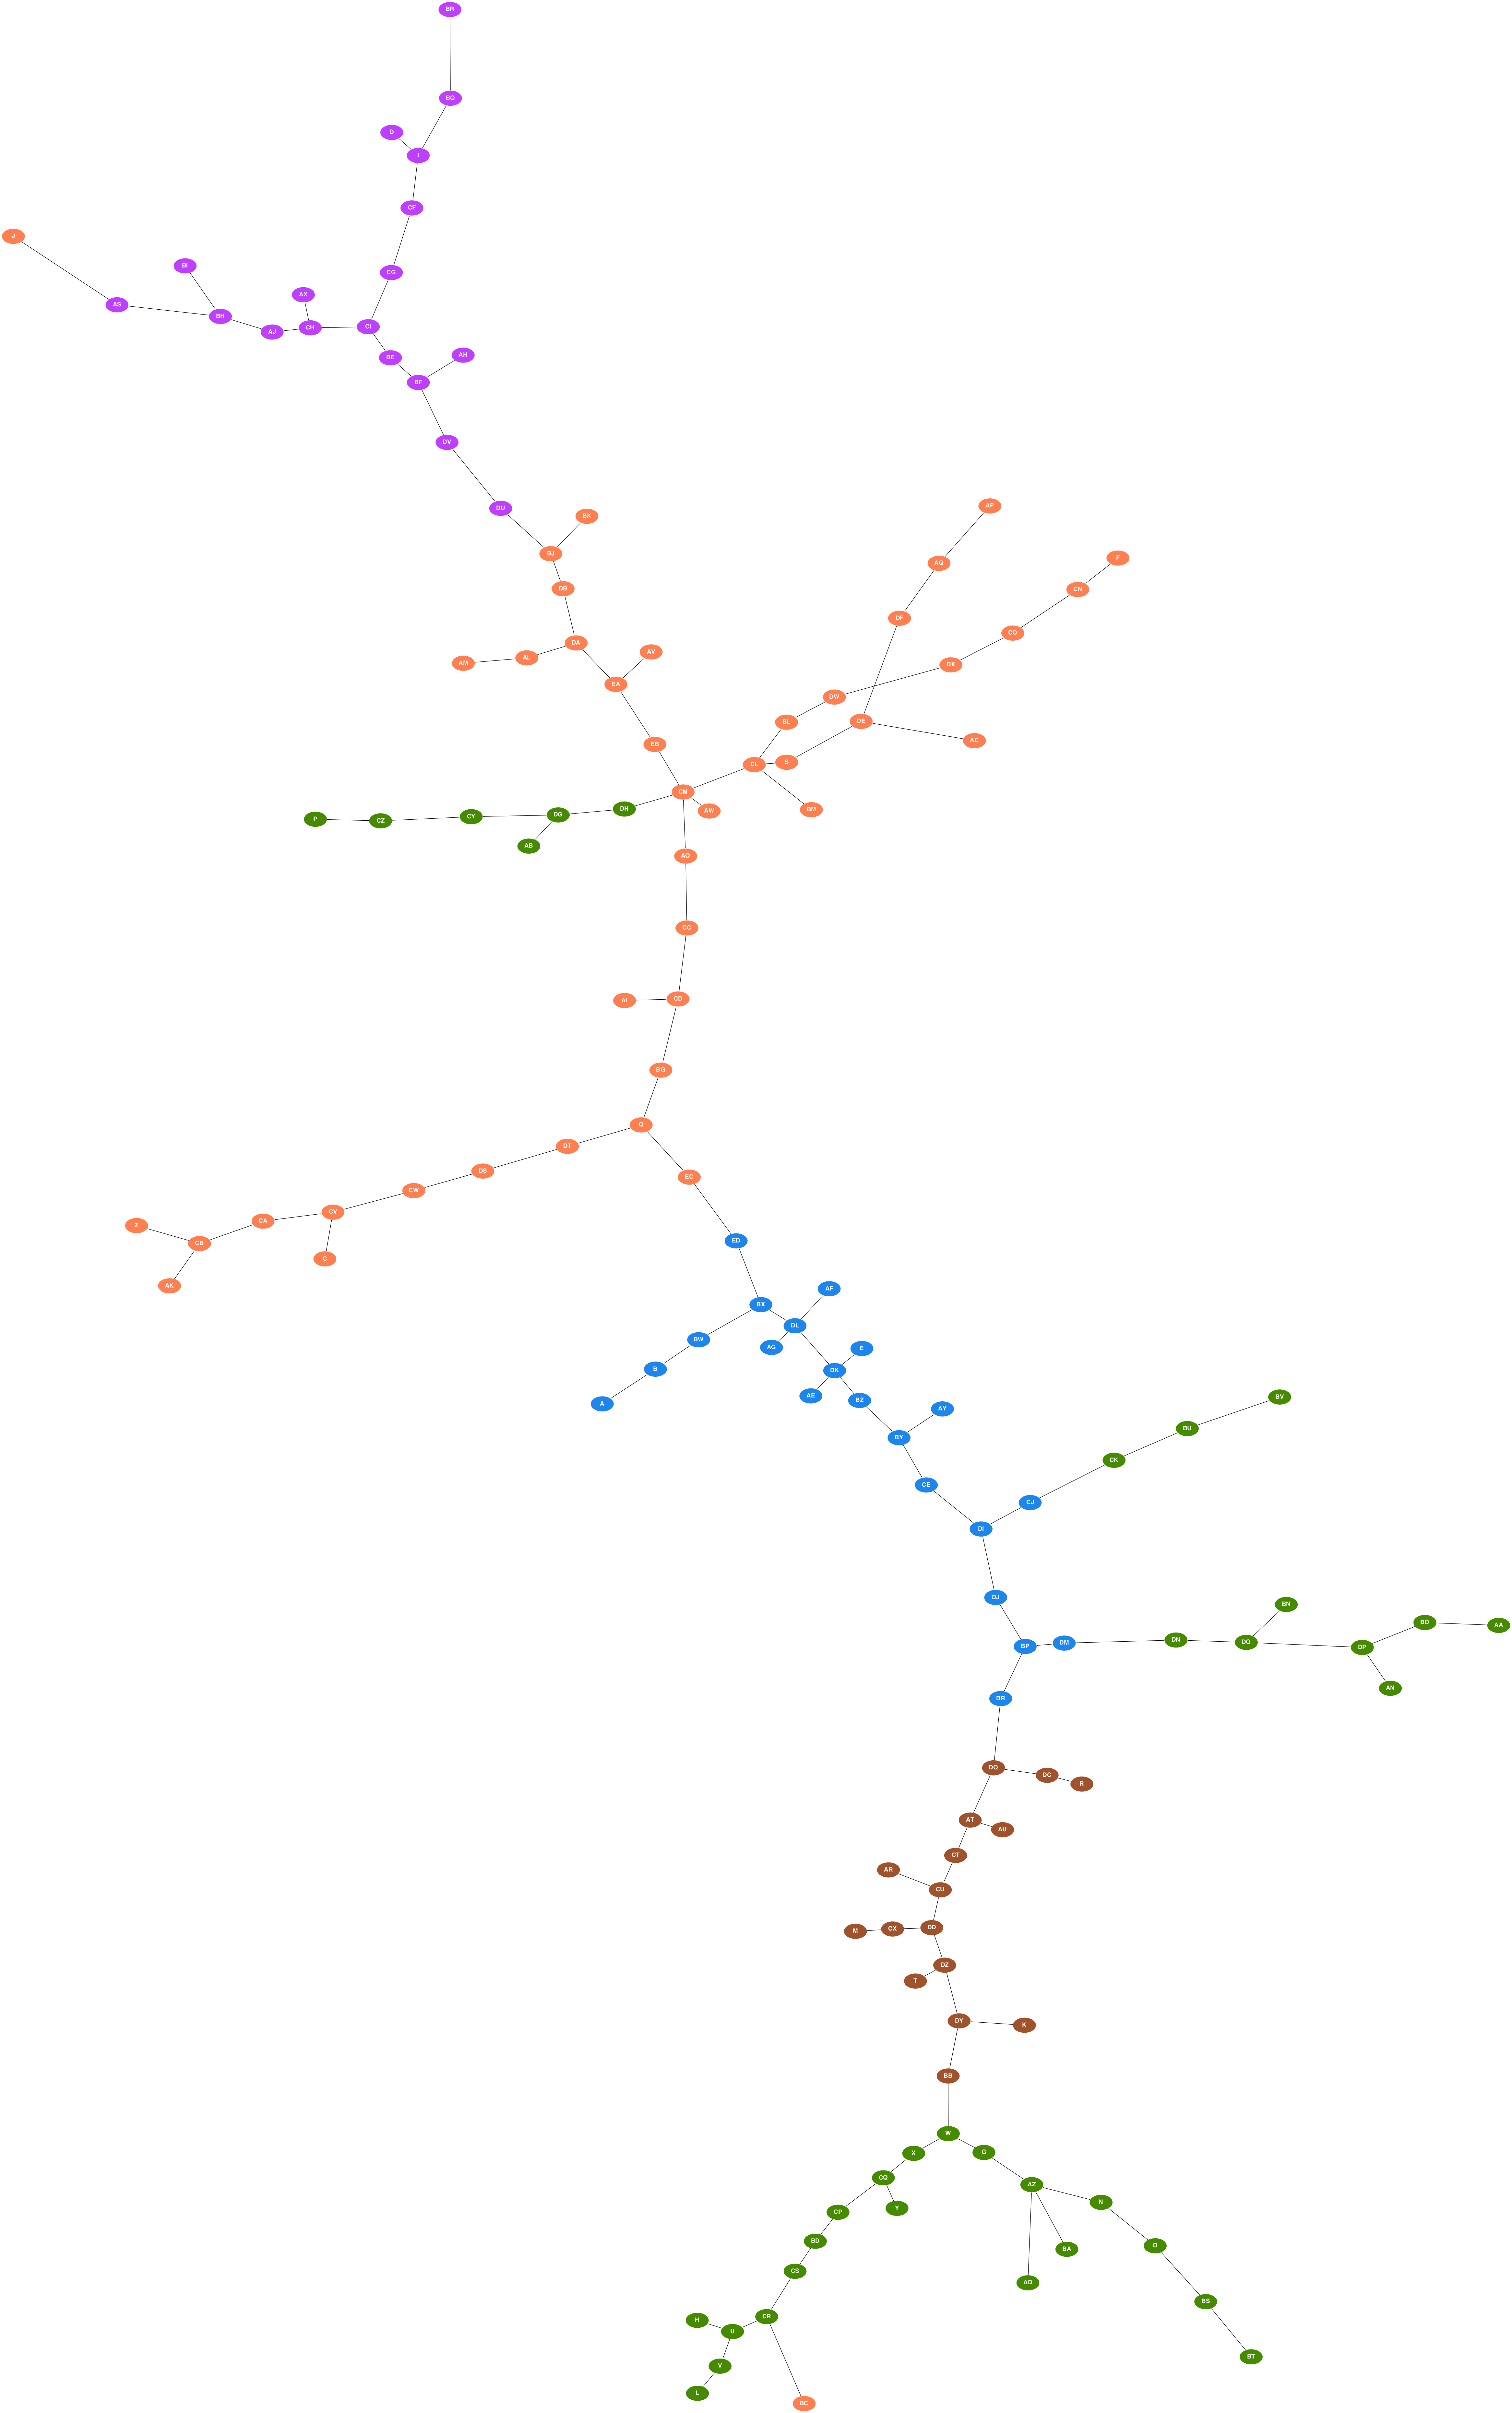
\includegraphics[width=\columnwidth-1cm]{img/mst1}
		\caption{MST from \textsl{test.dat} using Bor\r{u}vka's algorithm.}
		\label{fig:mst1}
	\end{center}
\end{figure}

Here also, the choice of Bor\r{u}vka's algorithm imposes itself.

\begin{lstlisting}[language=Lisp]
CL-MST> (neato (boruvka *distance-matrix*))
\end{lstlisting}

\begin{figure}[!hbt]
	\begin{center}
		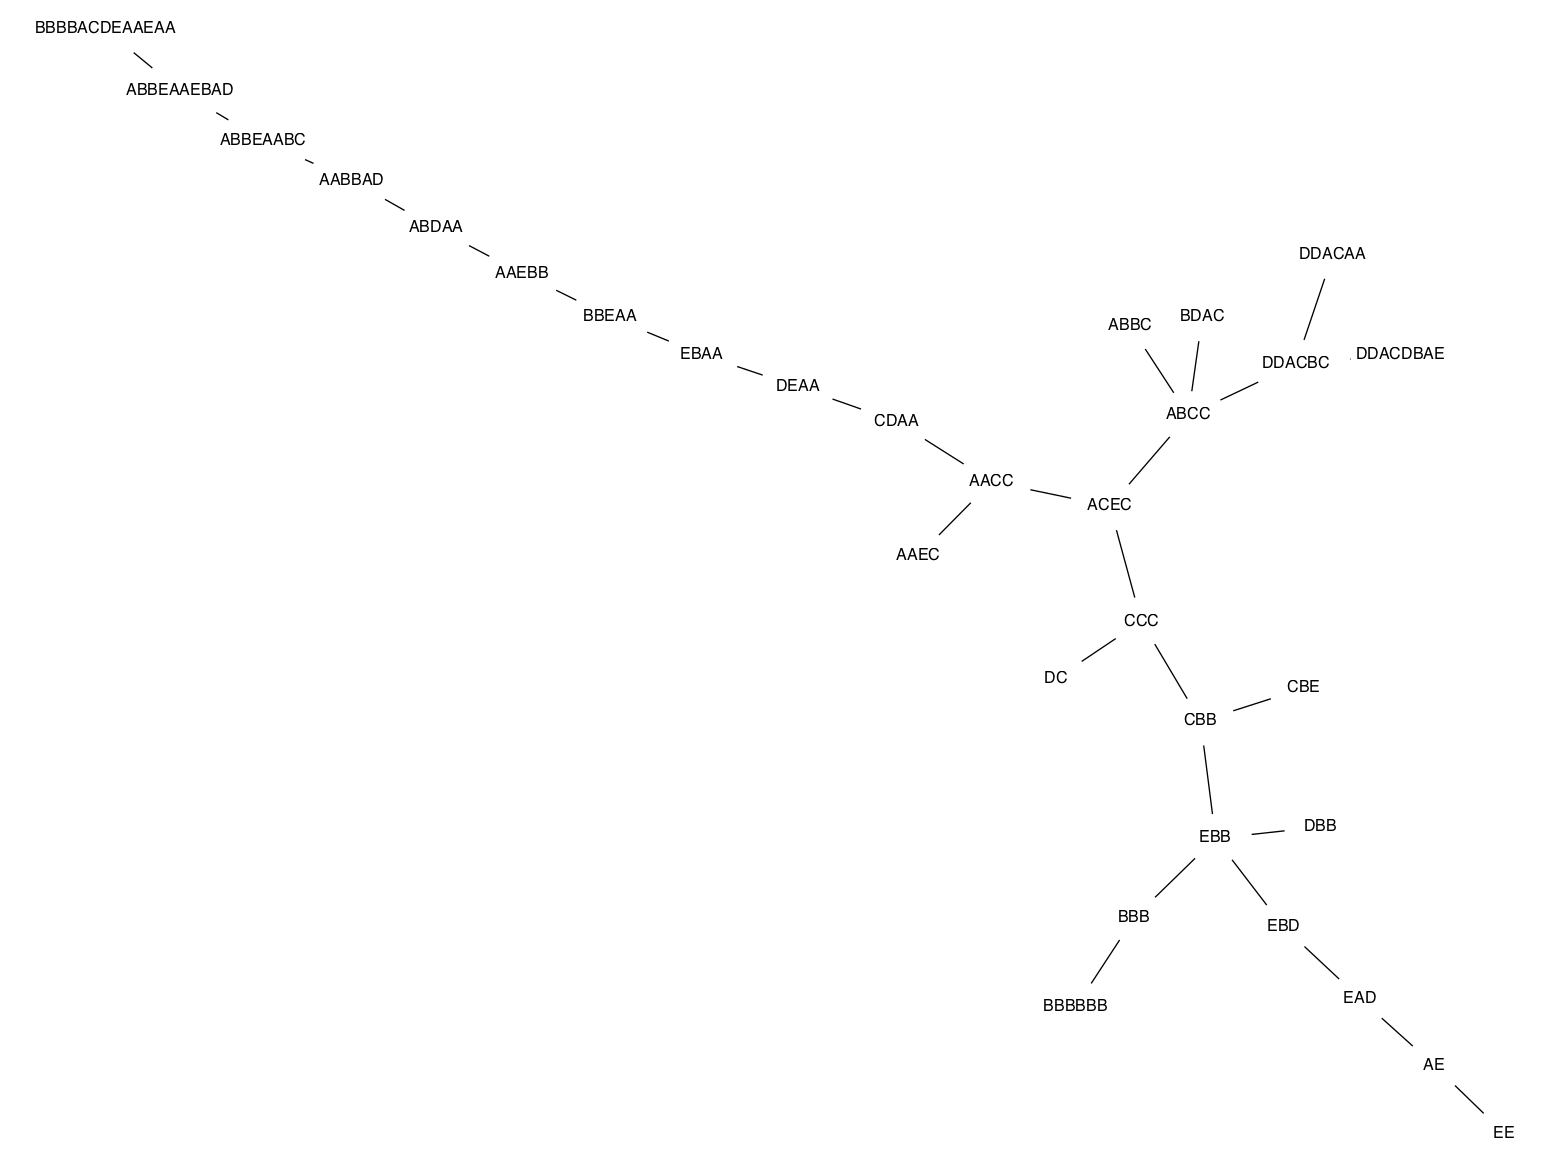
\includegraphics[width=\columnwidth]{img/mst2}
		\caption{MST of the contrastive clustering using Bor\r{u}vka's algorithm with the distance as described in the chapter \textsl{\nameref{paradigm}}.}
		\label{fig:mst2}
	\end{center}
\end{figure}

On the other hand, the MST in figure \ref{fig:mst2} offers an interesting view\footnote{Note for a better displaying of the graph, some attributes of the DOT file have been modified, as \texttt{overlap=compress} and \texttt{fontsize=12}.} as structural relationships, and a different approach for a paradigmatic discrimination. 

\smallskip

For instance, we can consider three branches from the node \textsf{ACEC}. Or even more relevant, we can cut the tree in two parts between the nodes \textsf{AACC} and \textsf{ACEC}, according to the branch defined by the path from \textsf{BBBBACDEAAEAA} to \textsf{AAEC}, and the branch defined by the path from \textsf{DDACDBAE} to \textsf{EE}.